\section{Kernel optimizations}

\begin{frame}[fragile]
\frametitle{Measure - Kernel initialization functions}
To find out which kernel initialization functions are the longest to
execute, add \code{initcall_debug} to the kernel command line.
Here's what you get on the kernel log:
\begin{block}{}
\tiny
\begin{verbatim}
...
[    3.750000] calling  ov2640_i2c_driver_init+0x0/0x10 @ 1
[    3.760000] initcall ov2640_i2c_driver_init+0x0/0x10 returned 0 after 544 usecs
[    3.760000] calling  at91sam9x5_video_init+0x0/0x14 @ 1
[    3.760000] at91sam9x5-video f0030340.lcdheo1: video device registered @ 0xe0d3e340, irq = 24
[    3.770000] initcall at91sam9x5_video_init+0x0/0x14 returned 0 after 10388 usecs
[    3.770000] calling  gspca_init+0x0/0x18 @ 1
[    3.770000] gspca_main: v2.14.0 registered
[    3.770000] initcall gspca_init+0x0/0x18 returned 0 after 3966 usecs
...
\end{verbatim}
\end{block}
It is probably a good idea to increase the log buffer size with
\code{CONFIG_LOG_BUF_SHIFT} in your kernel configuration. You will
also need \code{CONFIG_PRINTK_TIME} and \code{CONFIG_KALLSYMS}.
\end{frame}

\begin{frame}
\frametitle{Kernel boot graph}
With \code{initcall_debug}, you can generate a boot graph
making it easy to see which kernel initialization functions
take most time to execute.
\begin{itemize}
\item Copy and paste the console output or the output of
      the \code{dmesg} command to a file (let's call it \code{boot.log})
\item On your workstation, run the \code{scripts/bootgraph.pl} script
      in the kernel sources: \\
      \code{perl scripts/bootgraph.pl boot.log > boot.svg}
\item You can now open the boot graph with a vector graphics
      editor such as \code{inkscape}:
\end{itemize}
\begin{center}
    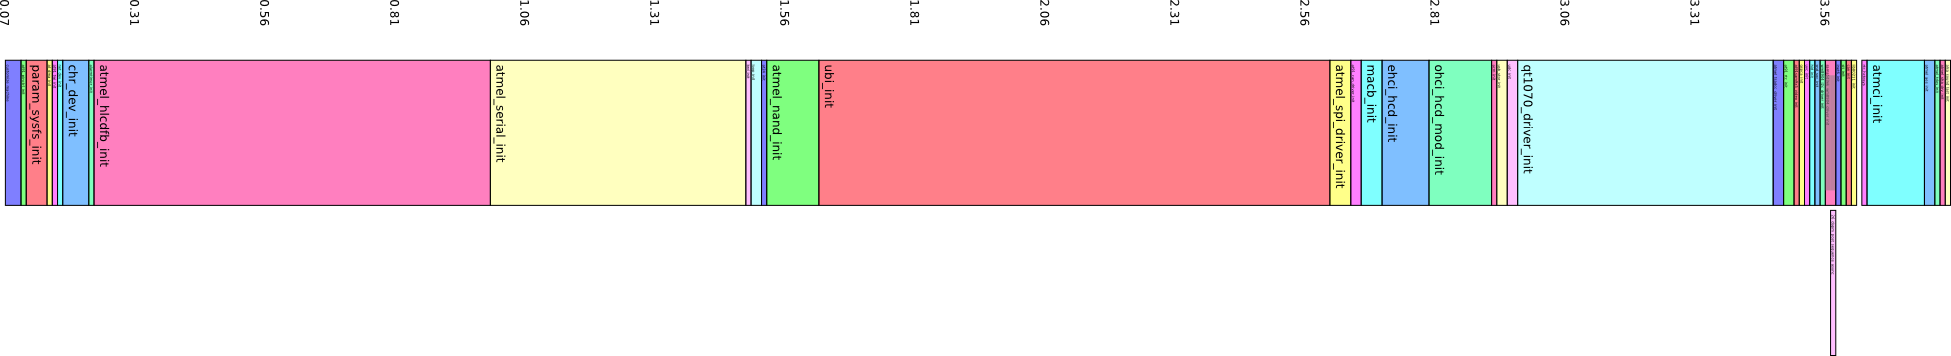
\includegraphics[width=\textwidth]{slides/boottime-kernel/boot.png}
\end{center}
\end{frame}

\begin{frame}
\frametitle{Using the kernel boot graph (1)}
Start working on the functions consuming most time first. For each
function:
\begin{itemize}
\item Look for its definition in the kernel source code. You can use LXR
      (for example \url{http://lxr.free-electrons.com}).
\item Remove unnecessary functionality:
      \begin{itemize}
      \item Look for kernel parameters in C sources and Makefiles, starting
      with \code{CONFIG_}. Some settings for such parameters could help
      to remove code complexity or remove unnecessary features.
      \item Find which module (if any) it belongs to. Loading this module
            could be deferred.
      \end{itemize}
\end{itemize}
\end{frame}

\begin{frame}
\frametitle{Using the kernel boot graph (2)}
\begin{itemize}
\item Postpone:
      \begin{itemize}
      \item Find which module (if any) the function belongs to.
            Load this module later if possible.
      \end{itemize}
\item Optimize necessary functionality:
      \begin{itemize}
      \item Look for parameters which could be used to reduce probe time,
            looking for the \code{module_param} macro.
      \item Look for delay loops and calls to functions containing
            \code{delay} in their name, which could take more time than
            needed. You could reduce such delays, and see whether the
            code still works or not.
      \end{itemize}
\end{itemize}
\end{frame}

\begin{frame}
\frametitle{Reduce kernel size}
First, we focus on reducing the size without removing features
\begin{itemize}
	\item The main mechanism is to use kernel modules
	\item Compile everything that is not needed at boot time as a
		module
	\item Two benefits: the kernel will be smaller and load faster, and
		less initialization code will get executed
	\item Remove features that are not used by userland:
		\code{CONFIG_KALLSYMS}, \code{CONFIG_DEBUG_FS},
		\code{CONFIG_BUG}
	\item Use features designed for embedded systems:
		\code{CONFIG_SLOB}, \code{CONFIG_EMBEDDED}
\end{itemize}
\end{frame}

\begin{frame}
\frametitle{Results}
Before:
\begin{center}
    \includegraphics[width=\textwidth]{slides/boottime-init-scripts3/timechart-initramfs.pdf}
\end{center}
After:
\begin{center}
    \includegraphics[width=\textwidth]{slides/boottime-kernel/timechart-modules.pdf}
\end{center}
\end{frame}

\begin{frame}
\frametitle{Kernel Compression}
\small
Depending on the balance between your storage reading speed and your
CPU power to decompress the kernel, you will need to benchmark
different compression algorithms.

Before (gzip):
\begin{center}
    \includegraphics[width=\textwidth]{slides/boottime-kernel/timechart-modules.pdf}
\end{center}
After (LZO):
\begin{center}
    \includegraphics[width=\textwidth]{slides/boottime-kernel/timechart-lzo.pdf}
\end{center}
Conclusion: don't use LZO for now.
\end{frame}

\begin{frame}
\frametitle{Deferred initcalls}
\begin{itemize}
\item If you can't compile a feature as a module (e.g. networking or block
      subsystem), try \code{deferred_initcalls}.
\item Your kernel will not shrink but some initializations will be
      postponed. Once your critical application is ready, you can
      execute the remaining initcalls.
\item See \url{http://elinux.org/Deferred_Initcalls}
\end{itemize}
\end{frame}

\begin{frame}
\frametitle{Turning off console output}
\begin{itemize}
\item Console output is actually taking a lot of time (very slow device).
      Probably not needed in production. Disable it by
      passing the \code{quiet} argument on the kernel command line.
\item You will still be able to use \code{dmesg} to get the kernel
      messages.
\item Time between starting the kernel and starting the \code{init}
      program, on Atmel SAMA5D3 Xplained (ARM), Linux 3.10:
      \newline\newline
    \begin{tabular}{| l || c | c | c |}
    \hline
    & Time & Diff \\
    \hline
    Without \code{quiet} & 2.352 s & \\
    With \code{quiet} & 1.285 s & -1.067 s\\
    \hline
    \end{tabular}
      \newline
\item Less time will be saved on a reduced kernel, of course.
\end{itemize}
\end{frame}

\begin{frame}[fragile]
\frametitle{Preset loops per jiffy}
\begin{itemize}
	\item At each boot, the Linux kernel calibrates a delay loop (for
	      the \kfunc{udelay} function). This measures a number of loops per
	      jiffy ({\em lpj}) value. You just need to measure this once! Find
	      the \code{lpj} value in the kernel boot messages:
\begin{block}{}
\tiny
\begin{verbatim}
Calibrating delay loop... 262.96 BogoMIPS (lpj=1314816)
\end{verbatim}
\end{block}
	\item Now, you can add \code{lpj=<value>} to the kernel command
	      line:
\begin{block}{}
\tiny
\begin{verbatim}
Calibrating delay loop (skipped) preset value.. 262.96 BogoMIPS (lpj=1314816)
\end{verbatim}
\end{block}
	\item Tests on Atmel SAMA5D3 Xplained (ARM), Linux 3.10:
      \newline\newline
    \begin{tabular}{| l || c | c | c |}
    \hline
    & Time & Diff \\
    \hline
    Without \code{lpj} & 71 ms & \\
    With \code{lpj} & 8 ms & -63 ms\\
    \hline
    \end{tabular}
	\newline
	\item This calculation was longer before 2.6.39 (about 200 ms).
\end{itemize}
\end{frame}

\begin{frame}
  \frametitle{Multiprocessor support (SMP)}
  \begin{itemize}
	  \item SMP is quite slow to initialize
	  \item UP systems may be faster to boot
	  \item What you can try is to hotplug the other cores after your critical application has started
  \end{itemize}
\end{frame}

\setuplabframe
{Reduce kernel boot time}
{
\begin{itemize}
\item Recompile the kernel, switching to an initramfs
\item Use \code{initcall_debug} to find the biggest
      time consumers
\item Reduce the number of modules
\item Tune kernel command line parameters
\end{itemize}
}

\begin{frame}
\frametitle{Kernel Optimization results}
Before (gzip)
\begin{center}
    \includegraphics[width=\textwidth]{slides/boottime-kernel/timechart-modules.pdf}
\end{center}
After:
\begin{center}
    \includegraphics[width=\textwidth]{slides/boottime-kernel/timechart-final.pdf}
\end{center}
Without losing any functionality!
\end{frame}

\begin{frame}
\frametitle{Kernel: last milliseconds (1)}
To shave off the last milliseconds, you will probably want to remove
unnecessary features:
\begin{itemize}
        \item \code{CONFIG_PRINTK=n} will have the same effect as the
              \code{quiet} command line argument but you won't have
	      any access to kernel messages. You will have a
              significantly smaller kernel though.
        \item Try \code{CONFIG_CC_OPTIMIZE_FOR_SIZE=y}. This will have
              an impact on performance, you will have to benchmark.
\end{itemize}
\end{frame}

\begin{frame}
\frametitle{Kernel last milliseconds (2)}
More features you could remove:
\begin{itemize}
        \item Module loading/unloading
        \item Block layer
        \item Network stack
        \item USB stack
        \item Power management features
        \item \code{CONFIG_SYSFS_DEPRECATED}
        \item Input: keyboards / mice / touchscreens
        \item \code{CONFIG_LEGACY_PTY_COUNT} or the
              \code{pty.legacy_count} kernel parameter
\end{itemize}
\end{frame}

